\section{Problem Statement}
% \textcolor{Blue}{You should make a decision on the topic you want to achieve. \\
	% Energy Efficient Cloud Resources Allocation with Container-based Cloud Computing}\\
% \textcolor{Maroon}{General introduction of cloud computing and Energy Consumption problem}
% The energy consumption in a data center has become the major concern for a Cloud provider. 

% The energy wastage mainly comes from the unproportional use of server resources \cite{Barroso:2007jt}

% Server consolidation \cite{Zhang:2010vo} is the major strategy to resolve this issue. 
% It reduces the server energy consumption by gathering virtual machines (VMs) into a fewer 
% number of physical servers so that idle servers can be turned off. 
Cloud computing is a computing model offers a network of servers to their 
clients in a on-demand fashion. From NIST's definition \cite{Mell:2011jj}, \textit{"cloud computing is a model for enabling ubiquitous, convenient, on-demand network access to a shared pool of configurable computing resources (e.g., networks, servers, storage, applications and services) that can be rapidly provisioned and released with minimal management effort or service provider interaction."}

\begin{figure}
	\centering
	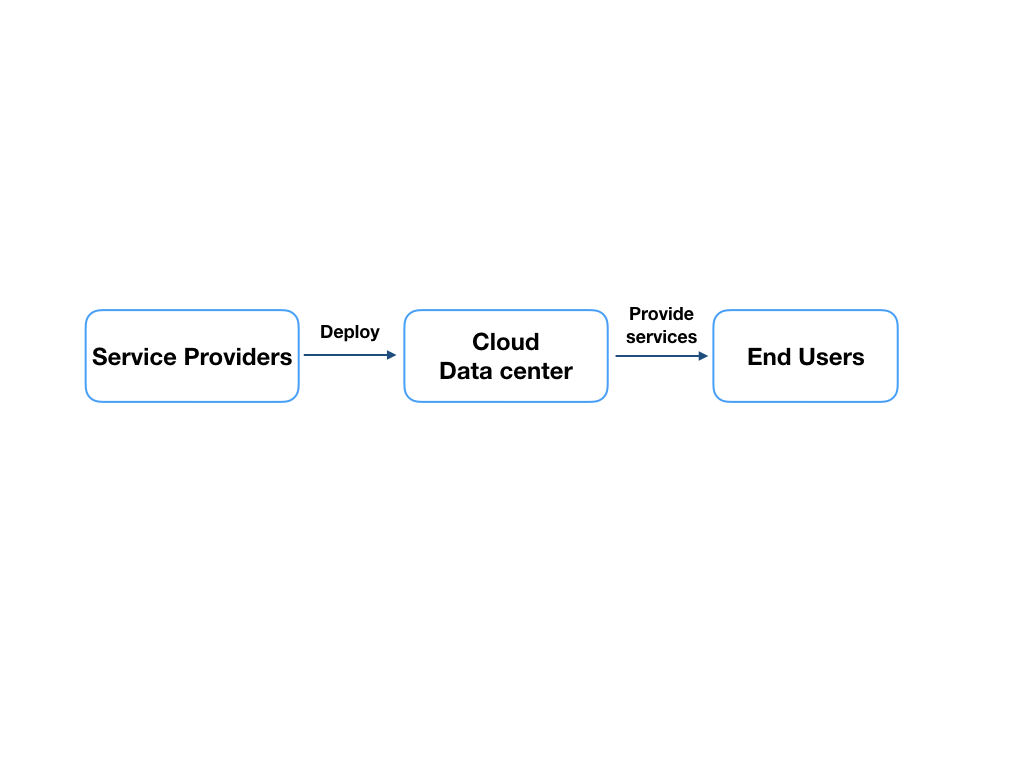
\includegraphics[width=0.7\textwidth]{pics/stakeholders.png}
	\caption{Stakeholders of Cloud computing}
	\label{fig:stakeholders}
\end{figure}

Cloud computing has completely reformed the software industry \cite{Buyya:2009ix} by providing three major benefits to web-based software or web service providers.
First, service providers do not need upfront investment in hardwares (e.g servers and networking devices) and pay for hardwares' maintenance. 


Second, service providers will not worried about the limited resources will obstruct the performance of their services when unexpected high demand occurs. The elastic nature of cloud can dynamic allocate and release resources for a service. In addition, software providers can pay as much as the resource usage under a \emph{pay-as-you-go} policy.
Third, service providers can publish and update their applications at any location 
as long as there is an Internet connection. 
These advantages allow anyone or organization to deploy their softwares on Cloud in
a reasonable price. 
% Cloud computing involves with three actors:
% \emph{Cloud provider}, \emph{Cloud users} and \emph{End users} 
% \cite{}. Cloud providers build and maintain the infrastructure of Cloud data centers. 
% Cloud users lease resources such as virtual machines from Cloud providers to deploy their applications so that end users can buy their services.

% The convenience offered by Cloud computing and the 
% difficulties of managing Cloud resources are two sides of a coin. 
From Cloud providers' perspective, they are trying to make the most profit on data centers.
On one hand, cloud providers are trying to improve the quality of  Cloud service to attract more service providers.  
On the other hand, they want to cut enormous energy consumption 
- as much as 25,000 households \cite{Kaplan:up01fR-k} - to lower the expense. 

Energy consumption in data centers are derived from several parts as 
illustrated in Figure \ref{fig:consumption}. 
Regardless the energy consumption of refrigeration system (or cooling system), 
the majority are from servers.
According to Hameed et al \cite{Hameed:2016cma}, 
servers are far from energy-efficient. 
The main reason for the wastage is that the energy consumption of servers remains high even when the utilization are low. Therefore, a concept of
\emph{energy proportional computing} \cite{Barroso:2007jt} raised to address the disproportionate between utilization and energy consumption. This leads to 
using vitualization technology to achieve server consolidation.
\begin{figure}
	\centering
	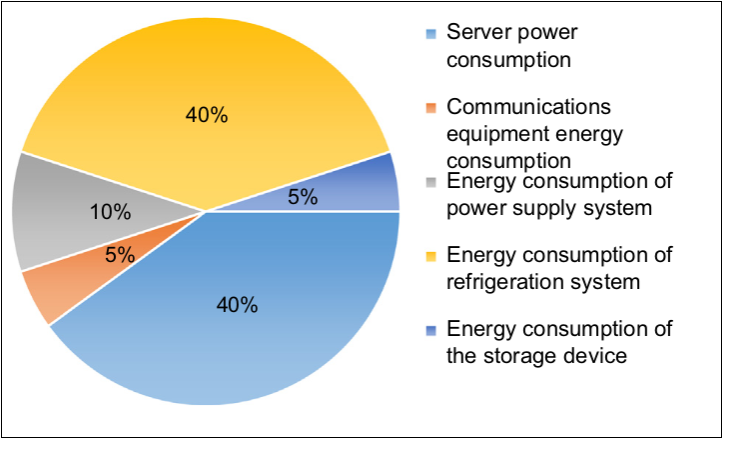
\includegraphics[width=0.5\textwidth]{pics/energyConsumption.png}
	\caption{Energy consumption distribution of data centers \cite{Rong:2016js}}
	\label{fig:consumption}
\end{figure}

Virtualization \cite{Uhlig:2005do} partitions a physical machine's resources (e.g. CPU, memory and disk) into several isolated units called virtual machines (VMs) where each VM allows an operating system running on them. This technology rooted back in the 1960s' and was originally invented to enable isolated software testing. Soon, people realized it can be a way to improve the utilization of hardware resources. Thereafter, a resource management strategy of server consolidation was invented.

Server consolidation \cite{Zhang:2010vo} resolves the low utilization problem by gathering virtual machines (VMs) into a fewer number of physical machines (PMs), so that the resource utilization of PMs are maintained at a high level. In the meanwhile, idle servers are turned off to save energy. Consolidation can minimize investments in hardware, hardware maintenance, data center space and energy consumption including both servers consume and cooling systems.

Despite the usefulness of server consolidation, it is a difficult task. 
Server consolidation is often considered as a global optimization problem 
where its goal is to minimize the overall energy consumption. 
It is often modeled as a bin-packing problem \cite{Mann:2015ua} which is a well-known NP-hard problem meaning it is unlikely to find an optimal solution 
of a large problem. Previous research have studied the problem extensively. 
Deterministic methods such as  
Integer Linear Programming \cite{Speitkamp:2010ck} and Mixed
Integer Programming \cite{Wang:2016eh} are unsuitable for a large scale problem 
because of the long computation time.  More research proposed heuristic methods
 to approximate the optimal solution such as 
First Fit Decreasing (FFD) \cite{Panigrahy:2011wk}, Best Fit Decreasing (BFD) \cite{Xu:2010vh}.
Manually designed heuristics are designed to tackle the special requirements such 
as a bin-item incomplete scenario \cite{Gupta:2008ul} and Multi-tier Applications \cite{Jung:2008vb, Li:2009wf}. Although these greedy-based heuristics can quickly solve the consolidation problem,  as Mann's research \cite{Mann:2015ua} shown, 
server consolidation is a lot more harder than bin-packing problem because of multi-dimension, many constraints. Therefore, a simple greedy-based heuristic (e.g FFD) leads to a bad performance and human designed heuristics cannot handle it well when Cloud environment has changed.

In addition, virtualization technology has evolved to allow finer granularity resource management.
A recent development of Container technique \cite{Soltesz:2007cu} has drove the attention of both industrial and academia.
Container is an operating system level of virtualization which means multiple containers can be installed in a same operating system (see Figure \ref{fig:comparison}). Each container provides an isolated environment for an application. In short, a VM is partitioned into smaller manageable units.
This new concept starts a new service model called Container as a Service (CaaS) \cite{Piraghaj:2015uf}. 
From Cloud customers' perspective, CaaS has advantages of both IaaS (Infrastructure as a Service) and PaaS (Platform as a Service) but without their disadvantages. On one hand - similar to PaaS - it frees the customers' from low level resource management so that they can focus on application development. On the other hand - similar to IaaS - it allows customers to customize their software environment without being constrained by platforms. 
From Cloud providers' perspective, CaaS allows Cloud providers to manage both the deployment of applications and resource allocation.
Hence, Cloud providers have a complete control of resources which may lead to a better utilization of resources. However the management difficulty also increases. 
Currently, vast amount of research focus on VM-based server consolidation, which can not be directly used on Contained-based Cloud.
This thesis, therefore, aims at providing an end-to-end solution for Container-based server consolidation which includes three stages: initialization, static container-based server consolidation and dynamic container placement.

\begin{figure}
	\centering
	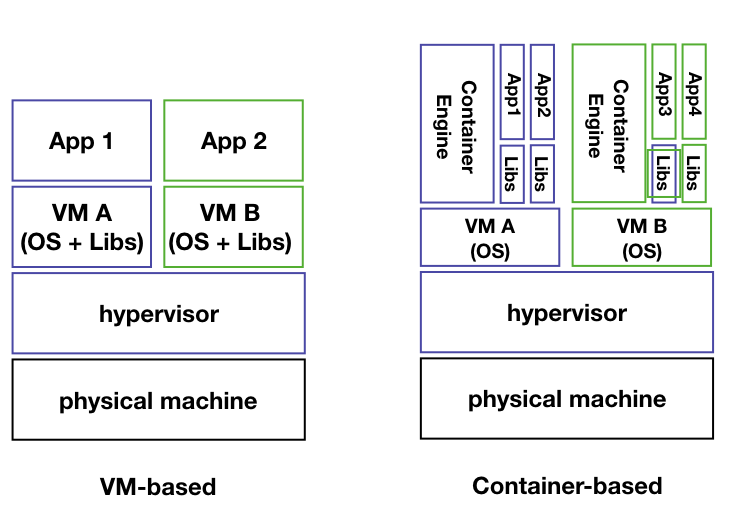
\includegraphics[width=0.7\textwidth]{pics/comparison.png}
	\caption{A comparison between VM-based and Container-based virtualization}
	\label{fig:comparison}
\end{figure}


% World Energy Outlook 2013 \cite{energyOutlook} estimated world electricity demand for 
% data centers was expected to increase by 66\% over the 2011 to 2035. 
% Beyond that, data centers also have an enormous impact on carbon 
% dioxide emissions \cite{2010arXiv1006.0308B}.


% % A well-accepted measurement: PUE (Power Usage Effectiveness) \cite{Belady:IMLoaM62}
% % a standard measurement for data center energy efficiency which compares the 
% % total power with the power used to power IT equipment (e.g. server, network equipments). 
% A recent survey \cite{Cho:2016kz} shows that the recent development of cooling techniques 
% have reduced its energy consumption and now 
% server consumption has become the dominate energy consumption component.
% Despite improvements in hardwares, various software techniques have been proposed 
% to reduce the energy consumption of servers 
% such as: Server Consolidation and Dynamic Voltage and Frequency Scaling (DVFS) \cite{}.

% Virtualization \cite{Uhlig:2005ub} is the core technology that not only enables 
% the elastic management of Cloud resource but also can be used to improve the utilization and reduce 
% energy consumption.
% It maps a physical machine's system resource - including processors, memory, and 
% other devices - into isolated units called \emph{Virtual Machines (VMs)} which allows 
% multiple operating system to run on. 
% In essence, virtualization add an extra layer of software called 
% \emph{Virtual Machine Monitor (VMM)} or \emph{hypervisors} that can deploy, 
% release and migrate VMs at runtime. 
% Numerous VMMs have been designed for x86 commodity machines such as 
% Xen \cite{Barham:2003vu}, KVM \cite{Kivity:2007wu}, and VMware ESX server \cite{Barham:2003vu}.
 
% \textcolor{Maroon}{A brief introduction of server consolidation}

% It aims at improving the income by guaranteeing \emph{Quality of Service (QoS)}
% \cite{Calheiros:2011ul} of the maximum number of applications that a datacenter can accommodate.

% The server consolidation techniques on the server-level
% have been extensively studied in the past decade \cite{}. 
% However, the recent development of container technology enables a VM-level of consolidation, which 
% has not driven much attention. 
% Container is a lightweight virtualization
% technology which allows an application running in a single container. 
% Multiple containers can be packed in a single virtual machine. 
% Two main advantages make the container popular. 
% First, containers do not need a Virtual Machine Monitor (VMM) but relies on the operating system; 
% it reduces the overhead used on managing the virtual system. 
% Second, the communication \cite{} between containers are much 
% easier (e.g. inter-process communication) than an inter-VM communication. This feature is 
% particularly useful for micro-service-based Web applications where their processes are packed
% into separated containers.
% This new technology has brought new challenges to server consolidation. 
% Traditional algorithms can not be directly applied since there is an extra level
% of virtualization. Affinity and communication aware allocation play an much important role 
% in container-based environment. Therefore, new techniques and algorithms are need to be proposed. 

% Currently, few literatures address the 

% Therefore, this thesis will focus on providing solutions to 
% container-based server consolidation.

% Mainly, there are two types of method: static and dynamic.
% Static methods are often treated as off-line approaches and applied in a periodical manner 
% where a batch of VMs are allocated to a set of servers. 
% They are conducted at a given point of time when
% the overall utilization in a data-center is degraded into a certain level: 
% e.g, a predefined CPU utilization threshold. Because static methods often consider partial or all VMs
% in a datacenter, it is often treated as a global optimization task \cite{}.
% The static method often models the problem as a off-line bin-packing problem and 
% solved with deterministic or heuristic algorithms. The goal is often to find a global optimal solution
% in terms of server utilization and other criteria.
% Dynamic method is an on-line approach. It assumes a scenario when a single server is 
% overloading with multiple VMs, migrate one of the internal VMs out from 
% the host will release the overloading. Dynamic method is used in between 
% two static consolidation processes to ease the overloaded server as well as consolidation.
% As it only moves one VM at a time, it often applies greedy-based heuristic, therefore, hard to 
% reach a global optimization.





% This thesis, therefore, aims at
% providing an end-to-end solution to the container-based server consolidation problem.

% First, aggressive consolidation causes overloading physical resources. 
% It leads to performance degradation since the application cannot obtain enough resources
% the VM promised. It is hard to determine the maximum level of utilization of a physical machine.